\documentclass[12pt]{exam}
\usepackage[version=4]{mhchem}
\usepackage[usenames,dvipsnames]{color}
\usepackage[T1]{fontenc}
\usepackage{tikz}
\usetikzlibrary{positioning}
\usetikzlibrary{arrows}
\usetikzlibrary{shapes.multipart}
\usepackage[caption=false]{subfig}
\usepackage{tabularx,tikz}
\usepackage{graphicx}
\usepackage{color}
\usepackage{pdfpages}

\pagestyle{headandfoot}
\runningheadrule
\firstpageheader{Name: \fillin[][4cm]}{Atomic Structure Notes}{Period \fillin[][1cm]}
\runningheader{Chemistry B}{Atomic Structure}{\today}
\firstpagefooter{}{}{}
\runningfooter{Chemistry B}{Atomic Structure, Page \thepage\ of \numpages}{\today}

\begin{document}

    
\begin{questions}

  \question 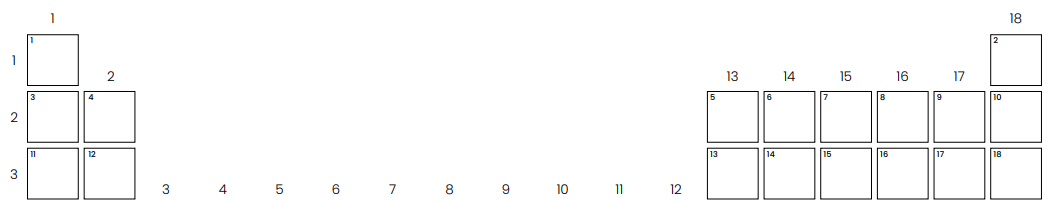
\includegraphics[width=15cm]{happytable.png}

  \noindent\rule{\textwidth}{1pt}

\end{questions}

\end{document}